\documentclass[a4paper]{article}

\usepackage[english]{babel}
\usepackage[utf8]{inputenc}
\usepackage{amsmath}
\usepackage{graphicx}
\usepackage{appendix}
\usepackage{longtable}
\DeclareGraphicsExtensions{.png}

\title{The Lost Vaults: Uneasy Alliance\\\small{An online multi-user Dungeon Client and Server.}\\\small{Project Proposal for group 4}}

\author{Felix Färjsjö\\(19911225-4678) \and Jimmy Holm\\(19870928-0138) \and Fredrik Larsson\\(19890422-0590) \and Anna Nilsson\\(19910804-0628) \and Philip Åkerfeldt\\(19920508-1335)}

\date{\today\\Version 2.0}

\begin{document}
\maketitle
\newpage
\begin{abstract}
A proposal for implementing a concurrent server model as the basis for an online, multi-user dungeon role playing game in Scala.
\end{abstract}

\tableofcontents
\listoffigures
\newpage
\section{Introduction}
Concurrency is becoming a more and more important facet of software development as computers rely more heavily on parallel processing and the way we write programs has to change to face 
the challenges that follow making use of this increase in processing power. As a way for us to explore these challenges and their solutions, we opted to work on a server-client 
system over a TCP/IP network connection. The problem we attempt to solve is maintaining a responsive environment for multiple, simultaneous connections as well as multiple active and 
independent sections of program logic. We represent this problem through a multi-user dungeon or MUD, a form of online multiplayer game, where we aim to make sure that the server maintains 
stable performance regardless of the number of connected users and we have decided to call this game Lost Vaults.

Lost Vaults is a semi-traditional MUD where users interact with other players and take on quests in parties 
of multiple players working towards a common goal while still looking out first and foremost for themselves. It is possible to adventure as a group of one person, but the focus of the 
game will be the group dynamic offered by interaction with other players. 
The game takes place in one of two locations, the city and the dungeon; the city being where the players may recoup from previous adventures, restock on supplies and 
form parties to delve back into the dungeon. The second location is the dungeon, a procedurally generated set of rooms populated with monsters, traps and treasures.
The dungeon is procedurally generated and instanced in such a way that each party of players has its own dungeon, uniquely generated when the party delves down into 
the magical caves underneath the city. Once inside, the party is given one or several quests they should take on while exploring.

A quest can be finding an object and bringing it back to the surface, killing a number of monsters or collecting a set amount of gold. The party works together to accomplish 
the goals, but at the same time only one of the party members reaps the rewards, making the party a tense and fragile alliance of rogues. Gold earned in the dungeon can be 
spent in the city on equipment and consumables to increase the player’s chance of surviving in the dungeon and taking on more difficult and threatening monsters.

The final product of this project will be a fully functional and interactive multiplayer online role playing game called The Lost Vaults.

The relation between the concept of concurrency and our project is the ability to have more than one player active in the game at the same time and their interaction with each other.
\part{Design}
\section{System Architecture}
The system architecture is in this document divided into  Client-side architecture and Server-side architecture. Being written in Scala, the application runs in the Java Virtual Machine and 
as such, both client and server should be able to run on any platform supporting Java VM 1.7.
\begin{figure}[hbt]
\centering
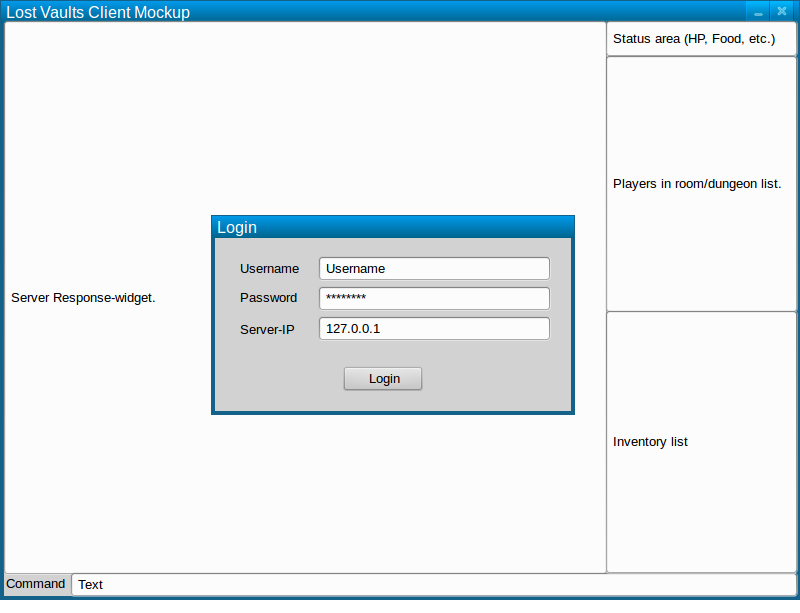
\includegraphics[width=1.0\textwidth]{clientmockup}
\caption{\label{fig:Client}User Interface mockup of the Lost Vaults Client.}
\end{figure}
\subsection{Client-side}
The design goal for the Lost Vaults client is to create something akin to a remote terminal, where no logic is performed beyond sending requests, and receiving and interpreting request responses. Ultimately, we aim to accomplish a client-side implementation that is easily extensible when the server's implementation of game logic increases, i.e. a system we can add to by simply adding new requests and responses.

As seen in Figure \ref{fig:Client} the client window is divided into several text areas displaying relevant information to the player. The main area is for regular server responses and will contain room descriptions, player chat messages, system information messages and similar.
The right side of the client is reserved for persistent information that the player may need to quickly reference. The top division contains information about the player's own character, listing the player's health and combat stats as well as the group's remaining food.

The bottom of the window contains the command input field, where the player types in commands in accordance to a strict syntax listed under the server architecture below.
Upon starting the client, the player is faced with the login window shown in the center of the mockup, where the player can enter their username and password as well as the server IP address to connect to.

The client GUI will be implemented using Java's Swing UI library and integrated into Scala to utilize Akka's TCP capabilities.
\subsubsection{Class Model}
The client is structured up into four distinct classes as described by figure \ref{fig:ClientArch}. The classes PlayGame and PlayGameCommunication work together to create a bridge between the TCP layer and the GUI, with PlayGame accepting messages from TCPClient and passing it along to the GUI through PlayGameCommunication. 
Likewise, the GUI sends data over the network  using method calls in PlayGameCommunication which passes it along to PlayGame and then TCPClient.
\begin{figure}[hbt]
\centering
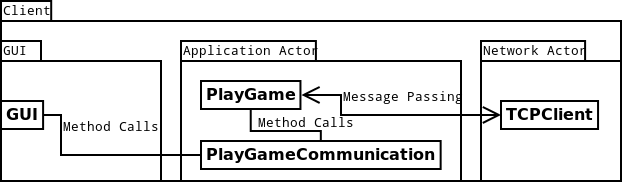
\includegraphics[width=1.0\textwidth]{clientuml1}
\caption{\label{fig:ClientArch}Client class relationship model.}
\end{figure}
\subsection{Server-side}
The server-side system architecture is further divided into the sections Concurrency model, Actor Model and Class Model. The first describes our choice of concurrency model and the 
reasoning behind it, the second describes  the function of the five major actor types of the Lost Vaults server and the final gives a more in-depth description of the 
class relationships used by the server.
\subsubsection{Concurrency Model}
We are opting to use the Actor Model for the project as we during our initial design discussion managed to isolate behaviour into several smaller and largely independent sections, 
which could with ease be made to share data only through message passing and thus avoiding the problem of deadlocks by removing shared data from the equation. 

In order to implement this kind of system with the greatest efficiency, we have chosen Scala as the language for the server as scalability is one of the fundamental design goals 
of the language. Per recommendation by the Scala language creators themselves and because of the library's strengths and ease of use, we decided to use Akka as our actor library and to make use of Akka's TCP 
library for network communication. Its simple integration also  guided our decision towards choosing Scala and Akka as the language and library of choice even for the client, as mentioned in the previous section.

\subsubsection{Actor Model}
\begin{figure}[ht]
\centering
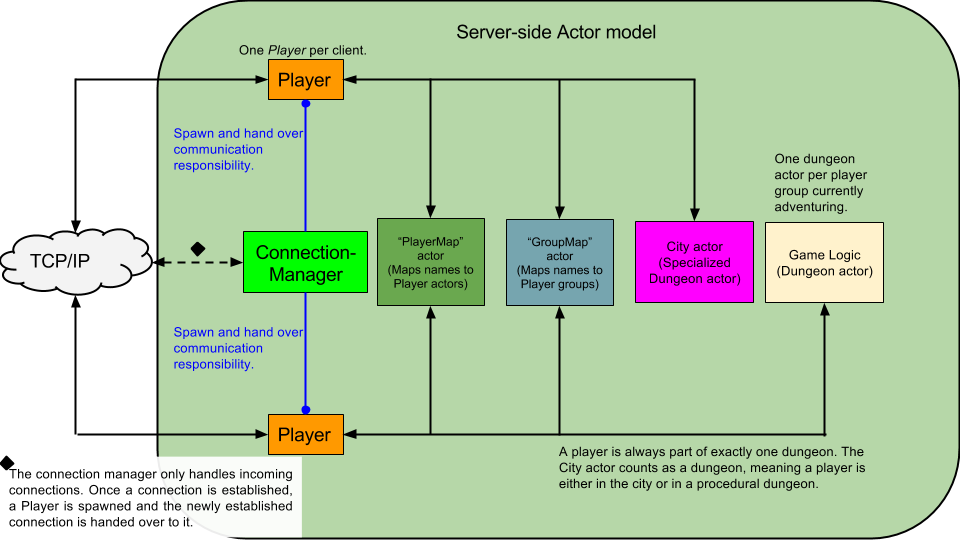
\includegraphics[width=1.0\textwidth]{serveractormodel}
\caption{\label{fig:ServerActorModel}Diagram of the server actors' interactions.}
\end{figure}
The server side is divided up into several processes using Akka's actor library to enforce the actor concurrency model in accordance with figure \ref{fig:ServerActorModel}. Only two types 
of actors communicate directly with the network through TCP/IP, the Connection Manager actor and the Player actors. The Connection Manager actor serves as the entry point for incoming
connections, and is in charge of spawning Player actors as new top-level actors before registering them as the newly established connection's listener. As the listener, the Player actor
will receive and send data over the network through the established connection. The Player actor is in charge of all things related to the clients, such as the specific player's attributes,
as well as verifying login attempts through communication with the PlayerMap and it is through the Player actors that the other actors can send messages over the network when necessary.

The PlayerMap actor and GroupMap actor serves two specific utility functions, the first of which is to map a string, the names of all connected players, to the actors controlling the player 
with that name. Through this actor, another actor can quickly and easily send messages to a specific actor based on its name - an important feature for commands acting on other players, 
such as \textit{WHISPER}. It also allows a quick and simple way for the Player actor to ensure no more than one player of a given name exists on the server at any given time.

The GroupMap actor performs a similar function as PlayerMap, however it links player names with player groups instead of player actors. A player group, as described in the game design 
section of this document, is a collection of one or more players who together can enter a dungeon that is procedurally generated for them. The purpose of this actor is to facilitate 
forming and joining other groups of players. Using the GroupMap, it is enough to join a player by name to be included into that player's group, or have a new group formed for them.

The fourth type of actor used by the Lost Vaults server is the Dungeon actor, the actor performing all game logic. There is a special case of Dungeon actor which is called the City actor. 
The City actor is a Dungeon actor that is persistent over the lifetime of the server and has special behaviour to handle the socializing aspect of chatting and forming groups as well as trading 
with NPC \footnote{Non-Playable Character} merchants. The ordinary case of the Dungeon Actor is in charge of generating and handling a procedural dungeon of multiple, interconnected rooms layed out in a two-dimensional 
grid. It is in these dungeon rooms that players will have the ability to complete quests, find treasure, etc. The Dungeon actor is in charge of coordinating all the players that are 
currently present in the dungeon, and make sure that commands such as \textit{SAY} are relayed to the relevant players. With the exception of the City actor, the Dungeon actors are 
in charge of their own lifespan after having been spawned by the City actor, and a Dungeon actor will stop itself once there are no more players within it.
\subsubsection{Class Model}
\begin{figure}[ht]
\centering
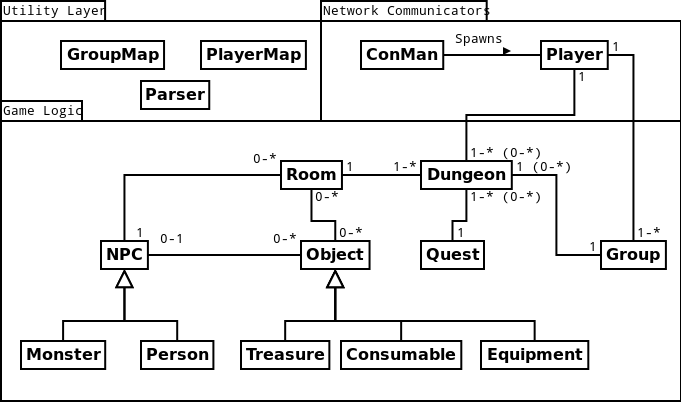
\includegraphics[width=1.0\textwidth]{serveruml1}
\caption{\label{fig:ServerUML}The server's class relationship model.}
\end{figure}
Figure \ref{fig:ServerUML} show the relationship between the different classes of the Lost Vaults server implementation and the multiplicity of relevant relationships. They are divided 
into three categories; the Utility Layer, the Network Communicators and the Game Logic. The Utility Layer provide supporting functionality to the other classes and exactly one of each 
class should exist at any given time. The Network Communicators are the ones that relate back to the network through Akka's TCP library. Of the two, ConMan, the connection manager class, 
is to be considered a singleton and only one instance should exist at any given time. The Player class however has one instance for each open connection.

The Game Logic section contains all the internal classes as well as the Dungeon class. The Dungeon class is the bridge between the Network Communicators and the Game Logic and it is 
only through a Dungeon class that a Player can perform any actions apart from the server-wide \textit{WHISPER} command. The Dungeon class keeps track of explored and unexplored rooms, 
quests, groups, objects and NPCs. The Dungeon also keeps track of all Players currently connected and associated with the given dungeon.
\section{Game Design}
[TODO: Describe game design here!]
\part{Development Process}
\section{Development Tools}
For this project we intend to use a number of tools to facilitate development.
Since we will be working in Scala we will be writing our code in Eclipse. We decided to use Eclipse because we consider it far the easiest way to develop code 
when writing in Java or Scala. Despite writing our code in Eclipse, however, we make use of the Ant build system to automate compilation and building of our client and server, ready
to be run in a Java virtual machine.
 
To handle version control we intend to use the reliable and well known tool Git. We setup a fresh git repository on GitHub.com specifically for this project and we chose 
Git because it is a powerful tool we are all familiar with.

Testing of our code will be done through the JUnit and ScalaTest frameworks and the Ant Build script will allow automatic building and running of the test suites.

For assembling our documentation we will use Scaladoc since it is similar to JavaDoc, a tool we are all familiar with and Ant has been amended to automatically build our documentations.

\section{Process evaluation}
We applied the Osborn principles for brainstorming with a small addition to the process. In the brainstorming process we went around the table and each group member had 
to add at least a couple of ideas before we let anyone who had an idea add them to the list of possible ideas. This led to many ideas which might lead to other group members 
coming up with new ideas from the proposed idea

The initial brainstorming went as expected with a long list of possible project ideas as the result. No ideas were criticised during the brainstorming and all the group members' 
ideas were shared. Nothing specific could be improved about our brainstorming session. 

During the brainstorming session three main project ideas were presented. The first idea was to make an online multiplayer game and the two others were simulation programs, 
one to simulate the traffic situation in a city and one to simulate an ecosystem. We divided the group into three focus groups that looked deeper into these three options. 
After this, each group were given time to present their respective fields, and after discussing pros and cons for the potential of each idea, we decided to choose the online 
multiplayer game. The reasons for this was that the complexity was intriguing, and that there was potential to develop the game further in case of extra time. Some of the 
interesting parts of the online game, besides being the most fun, was to learn about networking and our chosen programming language, Scala. 

Focusing on quantity in the first stage of brainstorming led to a good brainstorming process with plenty of ideas and doing so we found that it was easier to decide on a high 
quality idea when ideas could be put on the table and refined by the group as a whole, rather than feeling that any idea had to be fully formed before being suggested.

The main challenges that we expect to face during the development of both client and server are writing network code as well as learning a new programming language.
\newpage
\part{Appendices}
\begin{appendices}
\section{Network Messages}\label{app:NetworkMessages}
\begin{longtable}{|l|c|p{8 cm}|}
\hline
Message & Direction & Description\\
\hline
\endhead
\textit{SAY [msg]} & Client $\rightarrow$ Server & Chat message sent from client to server.\\
\hline
\textit{SAY [name] [msg]} & Client $\leftarrow$ Server & The Chat message sent by [name] and relayed to the relevant clients.\\
\hline
\textit{WHISPER [to] [msg]} & Client $\rightarrow$ Server & A private message sent from a player to another player named [to].\\
\hline
\textit{WHISPER [from] [to] [msg]} & Client $\leftarrow$ Server & A private message sent from a player named [from], to another player named [to].\\
\hline
\textit{LOGIN [name]} & Client $\rightarrow$ Server & A request to sign onto the server using [name] as the player's username.\\
\hline
\textit{LOGOUT} & Client $\rightarrow$ Server & A Request to sign out of the server.\\
\hline
\textit{LOGINOK} & Client $\leftarrow$ Server & Response from server that a login request has been accepted.\\
\hline
\textit{LOGINFAIL} & Client $\leftarrow$ Server & Response from server that a login request has been denied.\\
\hline
\textit{BYE} & Client $\leftarrow$ Server & Connection Closed message sent from server to client.\\
\hline
\textit{SYSTEM} & Client $\leftarrow$ Server & System mesage sent from the server to the client.\\
\hline
\textit{INVENTORY} & Client $\rightarrow$ Server & Request from a client to list a player's current inventory.\\
\hline
\textit{INVENTORY [list]} & Client $\leftarrow$ Server & Response to a client's inventory request. [list] is a comma delimited list of item names.\\
\hline
\textit{ROOMENTER [name]} & Client $\leftarrow$ Server & Notification that a player named [name] has entered the room which the client receiving the message is in.\\
\hline
\textit{ROOMLEAVE [name]} & Client $\leftarrow$ Server & Notification that a player named [name] has left the room which the client receiving the message is in.\\
\hline
\textit{ROOMLIST [list]} & Client $\leftarrow$ Server & Notification that the list of players in the client's current room should be repopulated. [list] is a newline-delimited list of names.\\
\hline
\textit{NPCLIST [list]}  & Client $\leftarrow$ Server & Notification that the list of NPCs should be updated. [list] is a newline-delimited list of NPC names.\\
\hline
\textit{ROOMITEMS [list]} & Client $\leftarrow$ Server & Notification of all the items in the current room. [list] is a newline- delimited list of all the items in the room.\\
\hline
\textit{ROOMDESC [description} & Client $\leftarrow$ Server & Notification of the client's current room's description.\\
\hline
\textit{ROOMEXITS [list]} & Client $\leftarrow$ Server & Notification of all possible exits from the client's current room.\\
\hline
\textit{ROOMPLAYERS} & Client $\rightarrow$ Server & Request for a list of players in the client's current room.\\
\hline
\textit{DUNGEONPLAYERS} & Client $\rightarrow$ Server & Request for a list of players in the client's current dungeon.\\
\hline
\textit{ROOMNPCS} & Client $\rightarrow$ Server & Request for a list of NPCs in the client's current room.\\
\hline
\textit{DESCRIBE} & Client $\rightarrow$ Server & Request for a room description of the client's current room.\\
\hline
\textit{ITEMS} & Client $\rightarrow$ Server & Request for a list of items in the client's current room.\\
\hline
\textit{EXITS} & Client $\rightarrow$ Server & Request for a list of exits in the client's current room.\\
\hline
\textit{HELP} & Client $\rightarrow$ Server & Request for a list of available commands and their descriptions.\\
\hline
\textit{DUNGEONENTER [name]} & Client $\leftarrow$ Server & Notification that a player named [name] has entered the same dungeon the client is currently in.\\
\hline
\textit{DUNGEONLEAVE [name]} & Client $\leftarrow$ Server & Notification that a player named [name] has left the room which the client receiving the message is in.\\
\hline
\textit{DUNGEONLIST [list]} & Client $\leftarrow$ Server & Notification that the list of players in the client's current room should be repopulated. [list] is a newline-delimited list of names.\\
\hline
\end{longtable}
\end{appendices}

\end{document}
